\documentclass[11pt,a4paper]{article}

% ---------------------------------------------------------------
% Rapport TP1 : Processus unifié et approches agiles
% Compilation : pdflatex rapport-tp1.tex (deux passes pour la table des matières)
% Texte et mise en forme sans couleur ; seuls les logos de la page de garde
% gardent leurs couleurs d'origine.
% ---------------------------------------------------------------

\usepackage[utf8]{inputenc}
\usepackage[T1]{fontenc}
\usepackage[french]{babel}
\usepackage{lmodern}
\usepackage[margin=2.3cm]{geometry}
\usepackage{graphicx}
\usepackage[export]{adjustbox}
\usepackage{booktabs}
\usepackage{tabularx}
\usepackage{array}
\usepackage{float}
\usepackage{enumitem}
\usepackage{listings}
\usepackage{amssymb}
\usepackage{microtype}
\usepackage[hidelinks]{hyperref}

\graphicspath{{figures/}}
\setlist{itemsep=2pt,topsep=4pt}
\setlength{\emergencystretch}{3em}
\newcolumntype{L}{>{\raggedright\arraybackslash}X}

% Listings en noir et blanc, avec prise en charge des accents
\lstset{
  basicstyle=\ttfamily\footnotesize,
  keywordstyle=\bfseries,
  commentstyle=\itshape,
  stringstyle=\ttfamily,
  columns=fullflexible,
  keepspaces=true,
  breaklines=true,
  frame=single,
  framerule=0.4pt,
  numbers=left,
  numberstyle=\tiny,
  xleftmargin=2em,
  showstringspaces=false,
  upquote=true,
  literate=
    {é}{{\'e}}1 {è}{{\`e}}1 {ê}{{\^e}}1 {ë}{{\"e}}1
    {à}{{\`a}}1 {â}{{\^a}}1 {ç}{{\c{c}}}1 {î}{{\^i}}1
    {ô}{{\^o}}1 {ù}{{\`u}}1 {û}{{\^u}}1
    {É}{{\'E}}1 {À}{{\`A}}1 {€}{{EUR}}3
    {«}{{\guillemotleft}}1 {»}{{\guillemotright}}1
    {—}{{---}}1 {–}{{--}}1 {≤}{{$\le$}}1 {→}{{$\rightarrow$}}1
}
\lstdefinelanguage{yaml}{
  keywords={name,on,push,pull_request,jobs,runs-on,steps,uses,with,run},
  sensitive=true,
  comment=[l]{\#},
}

\hypersetup{
  pdftitle={Compte rendu du TP n°1 : Processus unifié et approches agiles},
  pdfauthor={Mohamed Gharbi, Mohamed Louay Bourkhis, Soufien Hmaidi, Adem Yengui}
}

\begin{document}

% ---------------------------------------------------------------
% Page de garde
% ---------------------------------------------------------------
\begin{titlepage}
\centering
\begin{minipage}[c]{0.24\textwidth}
  \centering
  % Le PNG d'origine a une large marge blanche : on la coupe à l'affichage.
  \adjincludegraphics[width=\linewidth,trim={{.07\width} {.33\height} {.07\width} {.28\height}},clip]{logo-carthage.png}
\end{minipage}%
\hfill
\begin{minipage}[c]{0.48\textwidth}
  \centering\small
  République Tunisienne\\
  Ministère de l'Enseignement Supérieur\\
  et de la Recherche Scientifique\\[2pt]
  \textbf{Université de Carthage}\\
  \textbf{Institut National des Sciences}\\
  \textbf{Appliquées et de Technologie}
\end{minipage}%
\hfill
\begin{minipage}[c]{0.20\textwidth}
  \centering
  
\includegraphics[width=0.85\linewidth]{logo-insat.png}
\end{minipage}

\vspace{3cm}
\rule{\textwidth}{0.6pt}\\[0.6cm]
{\LARGE Compte rendu du TP n\textsuperscript{o}\,1}\\[0.4cm]
{\large Système de location de vélos et de trottinettes}\\[0.5cm]
\rule{\textwidth}{0.6pt}

\vspace{1cm}
{\large Matière : \textbf{Processus unifié et approches agiles}}\\[0.2cm]
{\large Filière : \textbf{RT4}}

\vfill
{\large\textbf{Réalisé par :}}\\[0.4cm]
Mohamed Gharbi\\
Mohamed Louay Bourkhis\\
Soufien Hmaidi\\
Adem Yengui\\[0.4cm]
RT4/2
\end{titlepage}

\begin{abstract}
Nous avons choisi un système de location de vélos et de trottinettes à six cas
d'utilisation (UC). Le plus risqué, \og Réserver un véhicule \fg{}, doit empêcher
deux clients de réserver le même véhicule sur des créneaux qui se chevauchent.
Le rapport suit l'ordre de l'énoncé. Il commence par le cadrage (vision,
priorisation, plan des itérations). Il décrit ensuite l'Élaboration, qui se termine
sur une première route exécutable et le tag \texttt{v0.1-elaboration}, puis la
Construction de cet UC : diagrammes UML, code en couches, 44 tests.
\end{abstract}

\tableofcontents
\newpage

% ===============================================================
\section{Choix du système}
% ===============================================================

Le système gère la location de vélos et de trottinettes en stations fixes. Il
compte six cas d'utilisation. L'UC à risque technique est UC2, Réserver un
véhicule : deux demandes peuvent viser le même véhicule sur des créneaux qui se
chevauchent, parfois au même instant.

\paragraph{Choix techniques.}
\begin{itemize}
  \item Langage et framework : Python 3.13, FastAPI 0.142.2.
  \item Accès aux données : SQLAlchemy 2.1.3 sur SQLite.
  \item Tests : pytest 9.1.1 (client de test HTTP via \texttt{httpx2}).
  \item Modélisation : PlantUML ; intégration continue : GitHub Actions.
  \item Gestion de version : Git (une branche par UC, jalons de phase sous forme de tags).
\end{itemize}

% ===============================================================
\section{Vision et acteurs (question 1)}
% ===============================================================

\subsection{Vision en cinq lignes}

\begin{enumerate}
  \item \textbf{Problème} : louer un vélo ou une trottinette en station se fait
        sans garantie de disponibilité ; doubles réservations et manque de
        visibilité frustrent les usagers.
  \item \textbf{Utilisateurs} : clients (étudiants, salariés, touristes) et
        opérateurs de flotte.
  \item \textbf{Valeur client} : réserver en ligne un véhicule sur un créneau
        garanti sans conflit, payer et restituer simplement.
  \item \textbf{Valeur opérateur} : visibilité sur la flotte, moins de litiges.
  \item \textbf{Périmètre} : API web, stations fixes, paiement via une passerelle
        externe simulée.
\end{enumerate}

\subsection{Acteurs}

\begin{table}[H]
\centering
\begin{tabularx}{\textwidth}{l l L}
\toprule
\textbf{Acteur} & \textbf{Type} & \textbf{Rôle} \\
\midrule
Client & principal & consulte, réserve, paie, annule, restitue \\
Opérateur de flotte & principal & gère les véhicules (ajout, retrait, maintenance) \\
Passerelle de paiement & secondaire (système externe) & autorise et capture les paiements \\
\bottomrule
\end{tabularx}
\caption{Acteurs du système}
\end{table}

% ===============================================================
\section{Liste des cas d'utilisation (question 2)}
% ===============================================================

\begin{table}[H]
\centering
\begin{tabularx}{\textwidth}{l l l L}
\toprule
\textbf{N\textsuperscript{o}} & \textbf{Cas d'utilisation} & \textbf{Acteur(s)} & \textbf{Description} \\
\midrule
UC1 & Consulter les véhicules disponibles & Client & lister les véhicules libres d'une station sur un créneau \\
UC2 & Réserver un véhicule & Client & bloquer un véhicule sur un créneau (UC à risque : conflits de réservation) \\
UC3 & Payer la location & Client, Passerelle & régler le montant via la passerelle externe \\
UC4 & Annuler une réservation & Client & libérer un créneau réservé \\
UC5 & Restituer le véhicule & Client & clore la location, calculer le prix final (inclut UC3) \\
UC6 & Gérer la flotte & Opérateur & ajouter, retirer, mettre en maintenance un véhicule \\
\bottomrule
\end{tabularx}
\caption{Cas d'utilisation}
\end{table}

% ===============================================================
\section{Priorisation des UC (question 3)}
% ===============================================================

Chaque UC reçoit une note de 1 (faible) à 3 (fort) pour la valeur métier (V), le
risque (R) et l'impact sur l'architecture (A).

\begin{table}[H]
\centering
\begin{tabular}{l c c c c l}
\toprule
\textbf{UC} & \textbf{V} & \textbf{R} & \textbf{A} & \textbf{Total} & \textbf{Itération} \\
\midrule
UC2 Réserver un véhicule          & 3 & 3 & 3 & \textbf{9} & It1 (Élaboration) \\
UC3 Payer la location             & 3 & 3 & 2 & 8 & It2 \\
UC1 Consulter les disponibilités  & 3 & 1 & 2 & 6 & It1 \\
UC5 Restituer le véhicule         & 2 & 2 & 2 & 6 & It2 \\
UC6 Gérer la flotte               & 2 & 1 & 2 & 5 & It3 \\
UC4 Annuler une réservation       & 2 & 1 & 1 & 4 & It3 \\
\bottomrule
\end{tabular}
\caption{Priorisation selon valeur métier, risque et impact architectural}
\end{table}

\paragraph{UC à traiter en premier.}
UC2 a la note maximale sur les trois critères. C'est lui qui fixe le modèle de
données, la gestion des transactions et la parade aux conflits, et les autres UC
s'appuient dessus. L'UP demande de traiter d'abord ce qui est risqué et structurant
pour l'architecture : UC2 passe donc en Élaboration. UC3 suit, parce qu'il dépend
d'un système externe, la passerelle de paiement.

% ===============================================================
\section{Planification : itérations, phases et jalons (question 4)}
% ===============================================================

\begin{table}[H]
\centering
\begin{tabularx}{\textwidth}{l l L l l}
\toprule
\textbf{Phase} & \textbf{Itér.} & \textbf{Contenu} & \textbf{Jalon} & \textbf{Tag} \\
\midrule
Lancement & cadrage & vision, acteurs, UC, priorisation, plan & LCO & \texttt{v0.0-lancement} \\
Élaboration & It1 & architecture de base exécutable : \texttt{POST /reservations} de bout en bout (UC2), CI verte & LCA & \texttt{v0.1-elaboration} \\
Construction & It2 & UC2 complet (règles, alternatives, concurrence), UC3, UC5 & aucun & aucun \\
Construction & It3 & UC4, UC6 & IOC & \texttt{v0.2-construction} \\
Transition & fin It3 & revue croisée, recette, documentation de déploiement & PR & \texttt{v1.0-transition} \\
\bottomrule
\end{tabularx}
\caption{Phases UP, itérations et jalons}
\end{table}

\noindent Signification des jalons :
\begin{itemize}
  \item \textbf{LCO} (\emph{Lifecycle Objectives}) : objectifs du cycle de vie validés ;
  \item \textbf{LCA} (\emph{Lifecycle Architecture}) : architecture de base stabilisée et \emph{exécutable} ;
  \item \textbf{IOC} (\emph{Initial Operational Capability}) : capacité opérationnelle initiale ;
  \item \textbf{PR} (\emph{Product Release}) : livraison du produit.
\end{itemize}

\noindent Les trois itérations :
\begin{itemize}
  \item \textbf{It1 (Élaboration)} : lever le risque technique ; livrer une route
        de bout en bout contrôleur $\rightarrow$ service $\rightarrow$ accès aux
        données pour UC2, avec un premier test automatisé en CI.
  \item \textbf{It2 (Construction)} : UC2 complet (fiche, classes, séquence, tests),
        puis UC3 et UC5.
  \item \textbf{It3 (Construction $\rightarrow$ Transition)} : UC4, UC6, revue croisée,
        stabilisation, livraison.
\end{itemize}

% ===============================================================
\section{Partie 1 : Élaboration}
% ===============================================================

\subsection{Dépôt, tableau de bord, tickets, milestones, branches et tags}

Le dépôt Git existe en local. Le script \texttt{github/setup-github.sh} le publie
sur GitHub une fois le dépôt distant créé : il crée les milestones, les tickets et
le tableau de bord, puis pousse les branches et les tags.

\paragraph{Tickets.} Chaque UC a son ticket (fichiers \texttt{github/issues/*.md}).
Trois tickets de plus suivent les livrables de phase :

\begin{table}[H]
\centering
\begin{tabular}{c l l}
\toprule
\textbf{Ticket} & \textbf{Titre} & \textbf{Milestone} \\
\midrule
\#1 à \#6 & UC1 à UC6 & Construction \\
\#7 & Lancement : vision, UC, priorisation, plan & Lancement \\
\#8 & Élaboration : architecture de base exécutable (UC2) & Élaboration \\
\#9 & Transition : revue croisée et livraison & Transition \\
\bottomrule
\end{tabular}
\caption{Tickets et milestones}
\end{table}

\paragraph{Milestones.} Un milestone par phase UP : Lancement, Élaboration,
Construction, Transition. Les tickets portent les labels \texttt{cas-utilisation},
\texttt{risque-technique} ou \texttt{phase}.

\paragraph{Tableau de bord.} Le script crée un \emph{GitHub Project} et y range
tous les tickets.

\paragraph{Branches.} Chaque UC possède sa branche :
\begin{itemize}
  \item \texttt{uc1-consulter-disponibilites}
  \item \texttt{uc2-reserver-vehicule}
  \item \texttt{uc3-payer-location}
  \item \texttt{uc4-annuler-reservation}
  \item \texttt{uc5-restituer-vehicule}
  \item \texttt{uc6-gerer-flotte}
\end{itemize}

\paragraph{Tags.} Chaque jalon de phase est un tag Git annoté. Nous avons posé
\texttt{v0.0-lancement} (LCO) et \texttt{v0.1-elaboration} (LCA) ;
\texttt{v0.2-construction} et \texttt{v1.0-transition} viendront aux jalons suivants.

\subsection{Diagramme de cas d'utilisation (PlantUML)}

La figure~\ref{fig:cas-utilisation} montre les trois acteurs et les six UC. UC5
inclut UC3 : rendre le véhicule déclenche le paiement. Source :
\texttt{docs/uml/cas-utilisation.puml}.

\begin{figure}[!htbp]
\centering
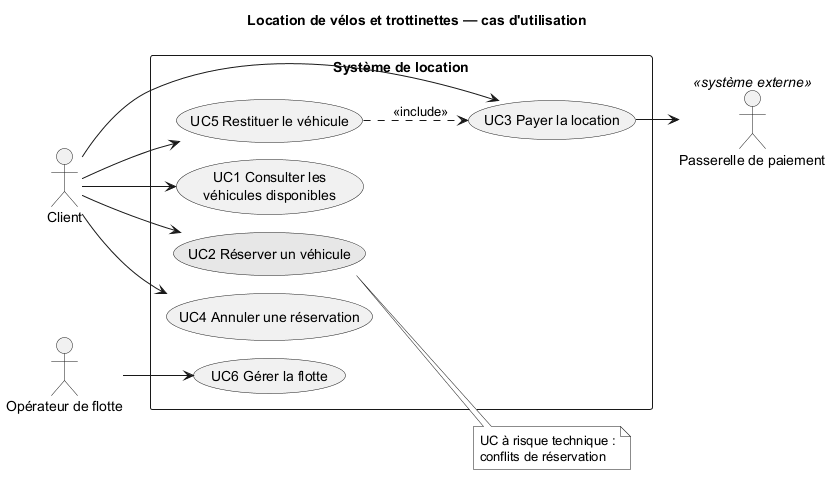
\includegraphics[width=0.9\textwidth]{cas-utilisation.png}
\caption{Diagramme de cas d'utilisation}
\label{fig:cas-utilisation}
\end{figure}

\subsection{Architecture de base exécutable}

Le code est découpé en quatre couches :

\begin{table}[H]
\centering
\begin{tabularx}{\textwidth}{l l L}
\toprule
\textbf{Couche} & \textbf{Emplacement} & \textbf{Rôle} \\
\midrule
Contrôleur & \texttt{app/api/reservations.py} & routes FastAPI, schémas Pydantic, HTTP $\leftrightarrow$ service \\
Service & \texttt{app/services/} & orchestration de l'UC, règles, transaction ; dépend de ports (\texttt{Protocol}) \\
Métier & \texttt{app/domain/} & objets purs : \texttt{Creneau}, tarif, énumérations, erreurs \\
Accès aux données & \texttt{app/repositories/}, \texttt{app/db.py}, \texttt{app/models.py} & dépôts et entités SQLAlchemy sur SQLite \\
\bottomrule
\end{tabularx}
\caption{Architecture en couches}
\end{table}

\paragraph{Route de l'UC à risque.}
\texttt{POST /reservations} passe par toutes les couches. Le contrôleur reçoit la
demande. \texttt{ReservationService} vérifie que le client et le véhicule existent,
puis que le créneau est libre. Le dépôt SQL enregistre la réservation.

\paragraph{Traitement du risque technique.}
La recherche de chevauchement et l'insertion se font dans la même transaction.
Celle-ci commence par \texttt{BEGIN IMMEDIATE}, qui prend tout de suite le verrou
d'écriture de SQLite. Si deux demandes arrivent en même temps, la seconde attend la
fin de la première, puis voit sa réservation et la refuse.

\begin{lstlisting}[language=Python,caption={\texttt{app/db.py} : transaction \texttt{BEGIN IMMEDIATE}}]
def creer_engine(url: str) -> Engine:
    engine = create_engine(url, connect_args={"check_same_thread": False, "timeout": 30})

    @event.listens_for(engine, "connect")
    def _desactiver_begin_implicite(connexion_dbapi, _enregistrement):
        connexion_dbapi.isolation_level = None

    @event.listens_for(engine, "begin")
    def _begin_immediate(connexion):
        connexion.exec_driver_sql("BEGIN IMMEDIATE")

    return engine
\end{lstlisting}

\paragraph{Premier test automatisé.}
Le premier test d'intégration,
\begin{center}
\texttt{test\_reserver\_creneau\_libre\_puis\_conflit},
\end{center}
\noindent vérifie qu'un créneau libre donne \texttt{201}, puis que le même créneau demandé
par un autre client donne \texttt{409 CONFLIT\_RESERVATION}.

\begin{lstlisting}[language=Python,caption={Premier test d'intégration}]
def test_reserver_creneau_libre_puis_conflit(client_http):
    premiere = client_http.post(
        "/reservations", json={"client_id": 1, "vehicule_id": 1, **CRENEAU_DEMAIN}
    )
    assert premiere.status_code == 201
    assert premiere.json()["statut"] == "CONFIRMEE"

    seconde = client_http.post(
        "/reservations", json={"client_id": 2, "vehicule_id": 1, **CRENEAU_DEMAIN}
    )
    assert seconde.status_code == 409
    assert seconde.json()["erreur"] == "CONFLIT_RESERVATION"
\end{lstlisting}

\paragraph{Intégration continue.} GitHub Actions lance les tests à chaque
\emph{push} et à chaque \emph{pull request}.

\begin{lstlisting}[language=yaml,caption={\texttt{.github/workflows/ci.yml}}]
name: CI

on:
  push:
  pull_request:

jobs:
  tests:
    runs-on: ubuntu-latest
    steps:
      - uses: actions/checkout@v4
      - uses: actions/setup-python@v5
        with:
          python-version: "3.13"
      - run: pip install -r requirements.txt
      - run: pytest -v
\end{lstlisting}

Nous avons aussi lancé l'application avec \texttt{uvicorn} et envoyé deux requêtes
à la main : la première réservation renvoie \texttt{201}, la seconde, sur le même
créneau, renvoie \texttt{409}.

\subsection{Tag \texttt{v0.1-elaboration} et fermeture du milestone}

Nous avons fusionné \texttt{uc2-reserver-vehicule} dans \texttt{main}
(\emph{merge} \texttt{--no-ff}, message \og Closes \#8, refs \#2 \fg{}). Les 13
tests passaient sur \texttt{main}, et nous avons posé le tag annoté
\texttt{v0.1-elaboration}. Le fichier \texttt{github/milestones.md} marque les
milestones Lancement et Élaboration comme fermés ; le script les fermera sur GitHub.
Le jalon LCA correspond donc à du code qui s'exécute et dont les tests passent.

% ===============================================================
\section{Partie 2 : Construction et Transition}
% ===============================================================

\subsection{Fiche UC2, diagramme de classes et diagramme de séquence}

\subsubsection*{Fiche UC2 : Réserver un véhicule}

\begin{table}[H]
\centering
\begin{tabularx}{\textwidth}{l L}
\toprule
Acteur principal & Client \\
Parties prenantes & Client (créneau garanti) ; Opérateur (pas de double réservation) \\
Préconditions & le client est identifié ; le véhicule existe \\
Garanties en cas de succès & une réservation \texttt{CONFIRMEE} est enregistrée avec son montant estimé ; aucune autre réservation confirmée ne chevauche ce créneau pour ce véhicule ni pour ce client \\
Garanties minimales & en cas d'échec, rien n'est enregistré \\
Déclencheur & le client choisit un véhicule (issu de UC1) et un créneau \\
\bottomrule
\end{tabularx}
\caption{En-tête de la fiche UC2}
\end{table}

\paragraph{Scénario nominal.}
\begin{enumerate}
  \item Le client envoie sa demande : identifiant client, identifiant véhicule, début, fin.
  \item Le système vérifie le créneau (début avant la fin, durée $\le$ 24 h, début dans le futur).
  \item Le système vérifie que le client et le véhicule existent.
  \item Le système vérifie que le véhicule n'est pas en maintenance.
  \item Le système vérifie qu'aucune réservation confirmée ne chevauche le créneau pour ce véhicule.
  \item Le système vérifie que le client n'a pas déjà une réservation confirmée sur ce créneau.
  \item Le système calcule le montant estimé (vélo 2~euros/h, trottinette 3~euros/h, toute heure entamée est due).
  \item Le système enregistre la réservation \texttt{CONFIRMEE} et la renvoie (HTTP 201).
\end{enumerate}

\paragraph{Scénarios alternatifs.}
\begin{itemize}
  \item \textbf{2a} Début $\ge$ fin ou durée $>$ 24 h $\rightarrow$ \texttt{CRENEAU\_INVALIDE} (422).
  \item \textbf{2b} Début $\le$ maintenant $\rightarrow$ \texttt{CRENEAU\_DANS\_LE\_PASSE} (422).
  \item \textbf{3a} Client ou véhicule inconnu $\rightarrow$ \texttt{CLIENT\_INTROUVABLE} / \texttt{VEHICULE\_INTROUVABLE} (404).
  \item \textbf{4a} Véhicule en maintenance $\rightarrow$ \texttt{VEHICULE\_INDISPONIBLE} (409).
  \item \textbf{5a} Créneau déjà réservé pour ce véhicule $\rightarrow$ \texttt{CONFLIT\_RESERVATION} (409).
  \item \textbf{6a} Le client a déjà une réservation qui chevauche $\rightarrow$ \texttt{CONFLIT\_CLIENT} (409).
\end{itemize}

\paragraph{Règles métier.} Les étapes 2 à 6 du scénario appliquent les règles
suivantes :
\begin{table}[H]
\centering
\begin{tabularx}{\textwidth}{l L}
\toprule
\textbf{Règle} & \textbf{Énoncé} \\
\midrule
R1 & \texttt{debut < fin} et durée $\le$ 24 h \\
R2 & \texttt{debut} strictement après l'instant courant \\
R3 & le client et le véhicule existent \\
R4 & le véhicule n'est pas \texttt{EN\_MAINTENANCE} \\
R5 & pas de chevauchement avec une réservation \texttt{CONFIRMEE} du véhicule \\
R6 & pas de chevauchement avec une réservation \texttt{CONFIRMEE} du client \\
\bottomrule
\end{tabularx}
\caption{Règles métier de UC2}
\end{table}

\noindent Deux créneaux $a$ et $b$ se chevauchent si et seulement si
$a.\mathit{debut} < b.\mathit{fin}$ et $b.\mathit{debut} < a.\mathit{fin}$.
Un créneau de 10\,h à 11\,h et un créneau de 11\,h à 12\,h ne se chevauchent donc pas.
Une date reçue sans fuseau horaire est lue en UTC, et l'API répond en UTC
(suffixe \texttt{Z}).

\subsubsection*{Diagramme de classes}

La figure~\ref{fig:classes-uc2} range les classes par paquetage : contrôleur,
services, métier, accès aux données et entités persistantes. Le service ne voit
les dépôts qu'à travers des interfaces.

\begin{figure}[!htbp]
\centering
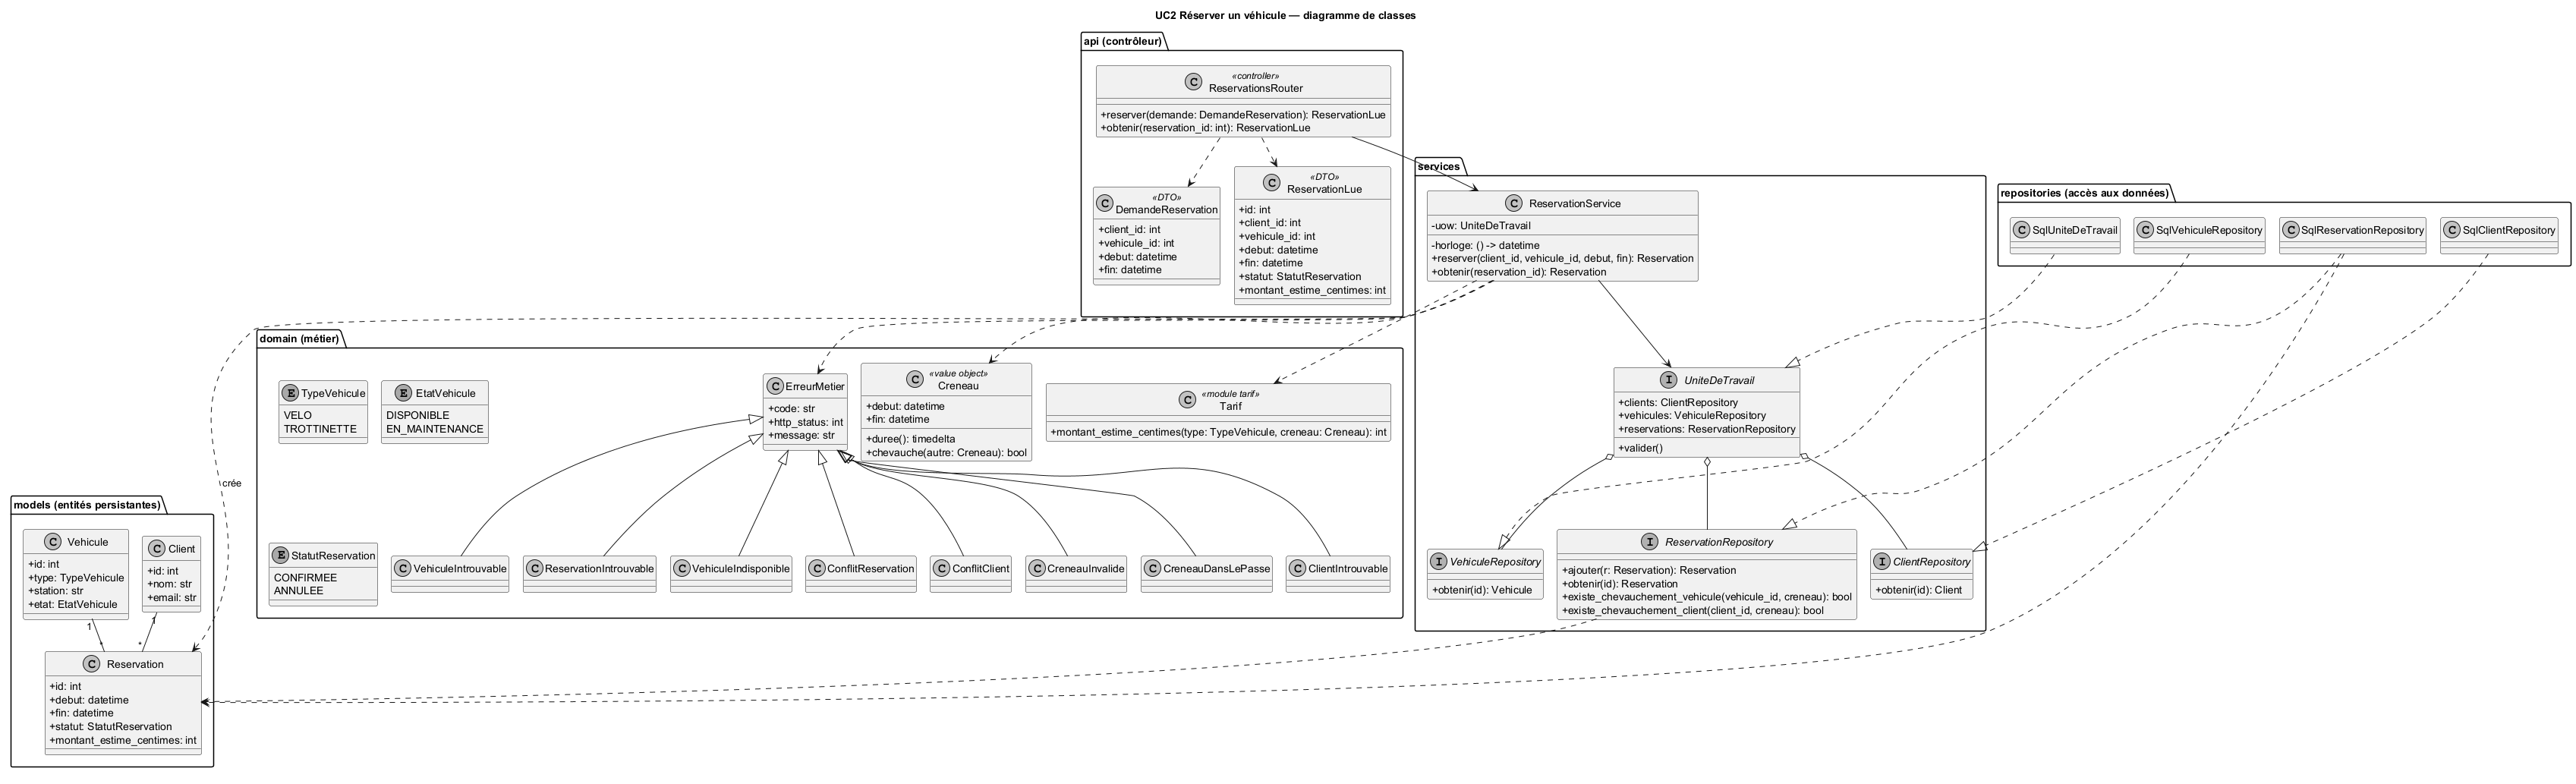
\includegraphics[width=\textwidth]{classes-uc2.png}
\caption{Diagramme de classes de UC2 (\texttt{docs/uml/classes-uc2.puml})}
\label{fig:classes-uc2}
\end{figure}

\subsubsection*{Diagramme de séquence (scénario nominal et alternative 5a)}

La figure~\ref{fig:sequence-uc2} suit une réservation du \texttt{POST} jusqu'au
\texttt{COMMIT}, puis montre l'alternative 5a : créneau déjà pris, annulation de la
transaction et réponse 409.

\begin{figure}[!htbp]
\centering
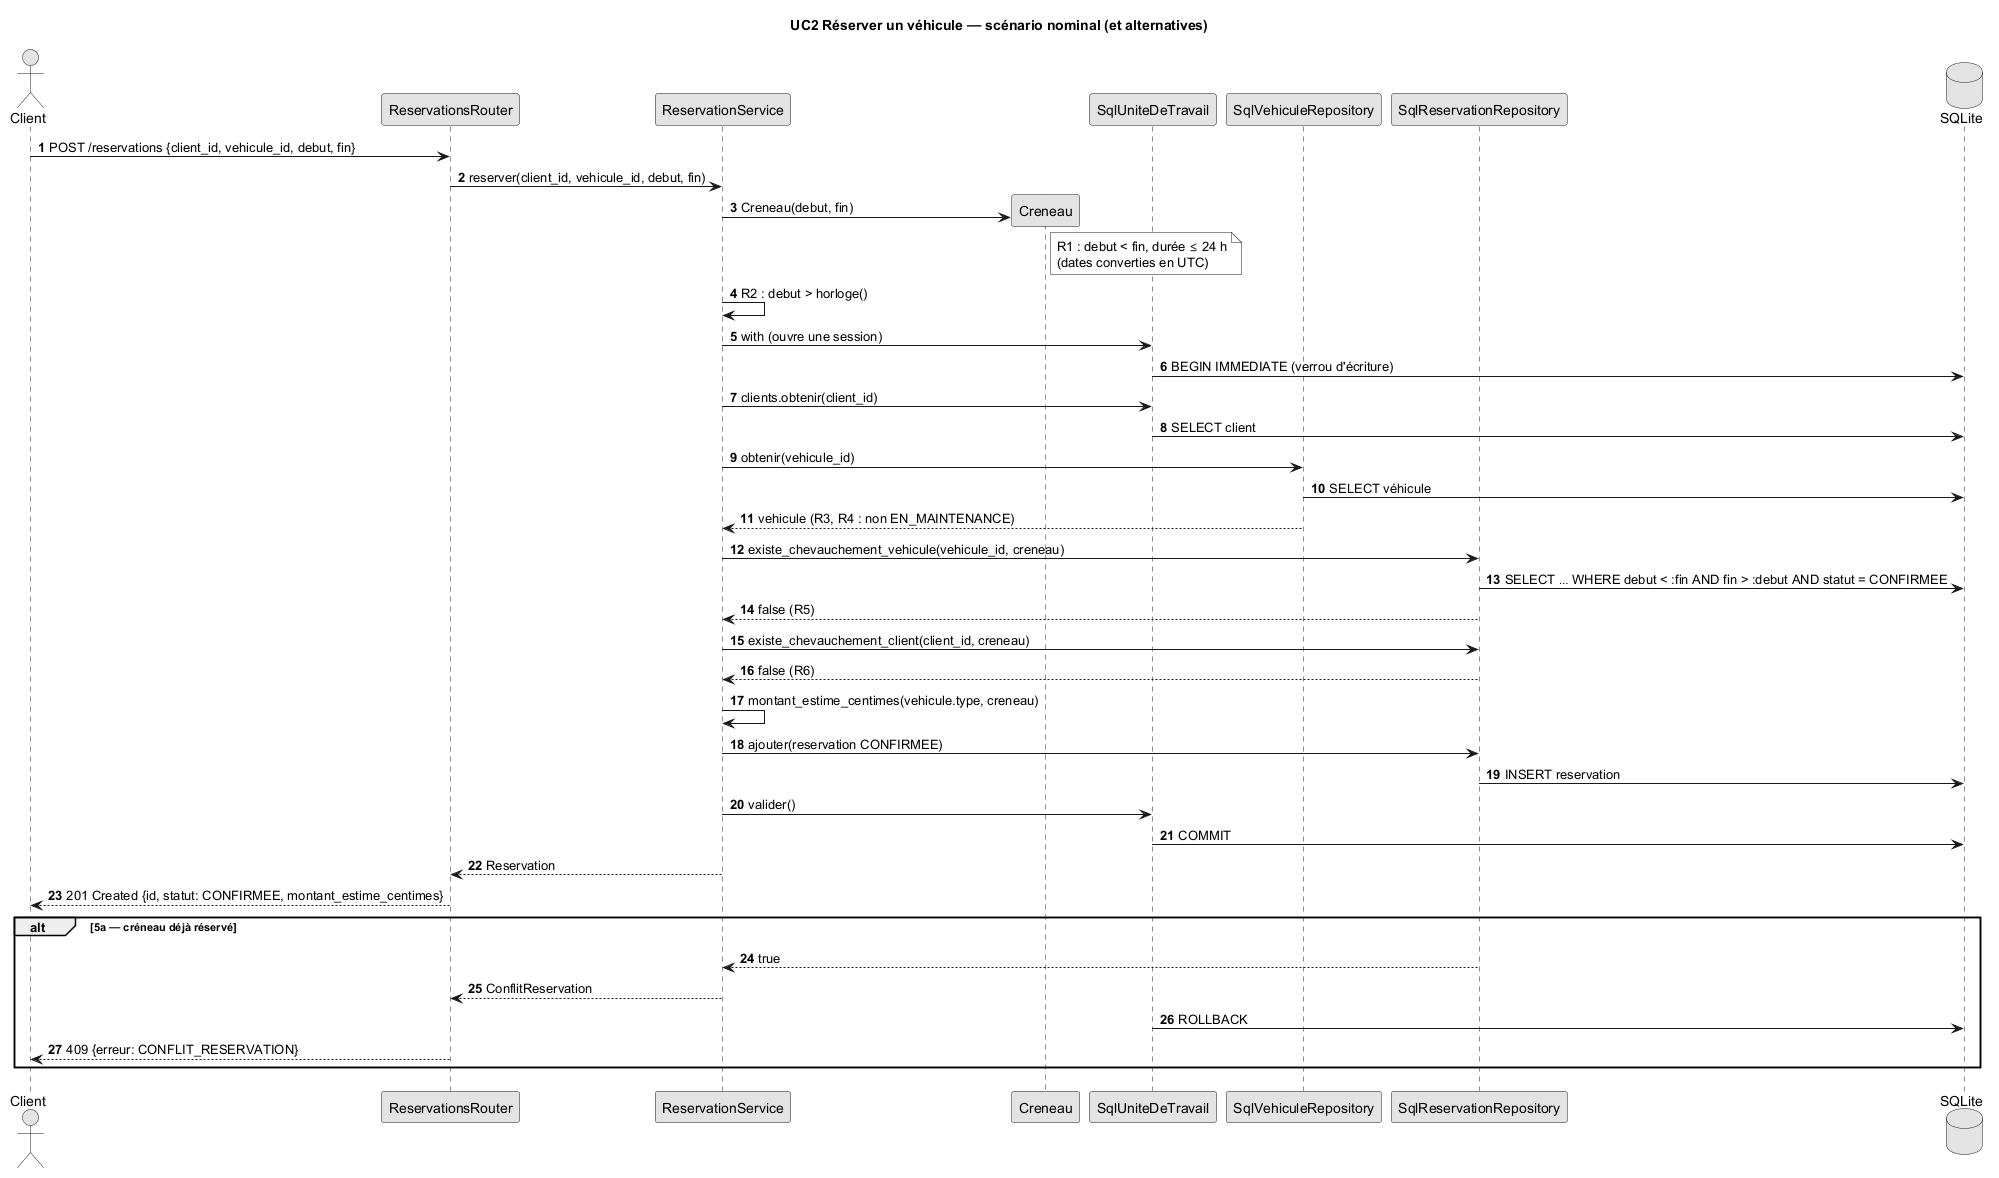
\includegraphics[width=\textwidth]{sequence-uc2.png}
\caption{Diagramme de séquence de UC2 (\texttt{docs/uml/sequence-uc2.puml})}
\label{fig:sequence-uc2}
\end{figure}

\subsection{Implémentation en couches (métier et accès aux données)}

\paragraph{Couche métier.} L'objet valeur \texttt{Creneau} convertit les dates en
UTC, applique R1 et sait dire si deux créneaux se chevauchent. Le module
\texttt{tarif} calcule le montant en centimes entiers, pour éviter les erreurs
d'arrondi des nombres flottants.

\begin{lstlisting}[language=Python,caption={\texttt{app/domain/creneau.py} (extrait)}]
@dataclass(frozen=True)
class Creneau:
    debut: datetime
    fin: datetime

    def __post_init__(self) -> None:
        object.__setattr__(self, "debut", en_utc_naif(self.debut))
        object.__setattr__(self, "fin", en_utc_naif(self.fin))
        if self.debut >= self.fin:
            raise CreneauInvalide("Le début du créneau doit précéder sa fin.")
        if self.duree > DUREE_MAX:
            raise CreneauInvalide("Un créneau ne peut pas dépasser 24 heures.")

    def chevauche(self, autre: "Creneau") -> bool:
        return self.debut < autre.fin and autre.debut < self.fin
\end{lstlisting}

\paragraph{Couche service.} \texttt{ReservationService} applique les règles R1 à R6
dans l'ordre de la fiche UC. Il reçoit une \emph{unité de travail} abstraite et une
horloge : les tests unitaires lui passent des faux dépôts en mémoire et une heure
fixe, sans base de données.

\begin{lstlisting}[language=Python,caption={\texttt{app/services/reservation\_service.py} (extrait)}]
def reserver(self, client_id, vehicule_id, debut, fin) -> Reservation:
    creneau = Creneau(debut, fin)  # R1
    if creneau.debut <= self._horloge():  # R2
        raise CreneauDansLePasse("Le créneau doit commencer dans le futur.")
    with self._uow as uow:
        if uow.clients.obtenir(client_id) is None:  # R3
            raise ClientIntrouvable(f"Client {client_id} introuvable.")
        vehicule = uow.vehicules.obtenir(vehicule_id)
        if vehicule is None:  # R3
            raise VehiculeIntrouvable(f"Véhicule {vehicule_id} introuvable.")
        if vehicule.etat == EtatVehicule.EN_MAINTENANCE:  # R4
            raise VehiculeIndisponible("Le véhicule est en maintenance.")
        if uow.reservations.existe_chevauchement_vehicule(vehicule_id, creneau):  # R5
            raise ConflitReservation("Le véhicule est déjà réservé sur ce créneau.")
        if uow.reservations.existe_chevauchement_client(client_id, creneau):  # R6
            raise ConflitClient("Vous avez déjà une réservation sur ce créneau.")
        reservation = Reservation(
            client_id=client_id, vehicule_id=vehicule_id,
            debut=creneau.debut, fin=creneau.fin,
            statut=StatutReservation.CONFIRMEE,
            montant_estime_centimes=montant_estime_centimes(vehicule.type, creneau),
        )
        uow.reservations.ajouter(reservation)
        uow.valider()
        return reservation
\end{lstlisting}

\paragraph{Couche d'accès aux données.} Le dépôt SQL écrit la règle de
chevauchement sous forme de requête. Les réservations annulées n'y comptent pas.

\begin{lstlisting}[language=Python,caption={\texttt{app/repositories/depots.py} (extrait)}]
def _existe_chevauchement(self, critere, creneau: Creneau) -> bool:
    requete = (
        select(Reservation.id)
        .where(
            critere,
            Reservation.statut == StatutReservation.CONFIRMEE,
            Reservation.debut < creneau.fin,
            Reservation.fin > creneau.debut,
        )
        .limit(1)
    )
    return self._session.scalar(requete) is not None
\end{lstlisting}

\paragraph{API.} L'API a deux routes. \texttt{POST /reservations} répond 201, 404,
409 ou 422 ; \texttt{GET /reservations/\{id\}} répond 200, 404 ou 422. Une erreur
métier renvoie :
\begin{center}
\texttt{\{"erreur": "<CODE>", "message": "..."\}}
\end{center}

\subsection{Tests unitaires et test d'intégration dérivés du scénario nominal}

Nous avons travaillé en TDD : chaque test est écrit avant le code qu'il couvre.
On le lance une première fois pour le voir échouer, puis on écrit juste assez de
code pour qu'il passe.

\begin{table}[H]
\centering
\begin{tabularx}{\textwidth}{l c L}
\toprule
\textbf{Fichier} & \textbf{Tests} & \textbf{Objet} \\
\midrule
\texttt{tests/unit/test\_creneau.py} & 11 & validation, chevauchement, créneaux contigus, durée max, conversion UTC \\
\texttt{tests/unit/test\_tarif.py} & 6 & heure entamée due, bornes (1 h + 1 \textmu s facturée 2 h) \\
\texttt{tests/unit/test\_reservation\_service.py} & 13 & scénario nominal et règles R1 à R6 avec faux dépôts en mémoire \\
\texttt{tests/integration/test\_depots.py} & 5 & requêtes SQL de chevauchement, réservations annulées ignorées \\
\texttt{tests/integration/test\_api\_reservations.py} & 8 & scénario nominal HTTP, erreurs, fuseaux horaires, entrées hors limites \\
\texttt{tests/integration/test\_concurrence.py} & 1 & deux réservations simultanées : un seul succès \\
\midrule
\textbf{Total} & \textbf{44} & tous passent \\
\bottomrule
\end{tabularx}
\caption{Répartition des tests}
\end{table}

\paragraph{Test unitaire du scénario nominal.} Le test appelle le service avec les
faux dépôts et une heure fixe. Il vérifie la réservation renvoyée, son montant et
l'appel à \texttt{valider()}.

\begin{lstlisting}[language=Python,caption={Test unitaire du scénario nominal}]
def test_scenario_nominal_enregistre_une_reservation_confirmee(service, uow):
    reservation = service.reserver(ALICE, TROTTINETTE, h(10), h(11, 30))

    assert reservation.id == 1
    assert reservation.statut == StatutReservation.CONFIRMEE
    assert reservation.montant_estime_centimes == 600
    assert uow.reservations.elements == [reservation]
    assert uow.valide
\end{lstlisting}

\paragraph{Test d'intégration du scénario nominal.} Il passe par toutes les couches
jusqu'à une base SQLite sur disque. Le client réserve (réponse 201 avec le montant),
puis relit la même réservation par \texttt{GET}.

\begin{lstlisting}[language=Python,caption={Test d'intégration du scénario nominal}]
def test_scenario_nominal_reserver_puis_consulter(client_http):
    reponse = client_http.post(
        "/reservations",
        json={"client_id": 1, "vehicule_id": 2,
              "debut": "2026-10-08T10:00:00", "fin": "2026-10-08T11:30:00"},
    )
    assert reponse.status_code == 201
    reservation = reponse.json()
    assert reservation == {
        "id": 1, "client_id": 1, "vehicule_id": 2,
        "debut": "2026-10-08T10:00:00Z", "fin": "2026-10-08T11:30:00Z",
        "statut": "CONFIRMEE", "montant_estime_centimes": 600,
    }

    consultee = client_http.get(f"/reservations/{reservation['id']}")
    assert consultee.status_code == 200
    assert consultee.json() == reservation
\end{lstlisting}

\paragraph{Test de concurrence (risque technique).} Deux fils d'exécution
réservent le même créneau au même moment, dix fois de suite. À chaque essai, l'un
doit réussir et l'autre recevoir un conflit. Pour vérifier que ce test détecte bien
le problème, nous avons remplacé \texttt{BEGIN IMMEDIATE} par \texttt{BEGIN} : le
test échoue (\texttt{database is locked}). Il repasse dès que le verrou est remis.
Pendant la relecture, un essai sans verrou a donné une double réservation dans 27
cas sur 28.

\subsection{Revue croisée}

\paragraph{Support fourni à l'équipe relectrice.}
\begin{itemize}
  \item \texttt{docs/revue/checklist-revue-croisee.md} : grille couvrant la
        traçabilité, le respect des couches, le traitement du risque de conflit et
        la qualité, avec un tableau de remarques à compléter ;
  \item \texttt{docs/revue/pr-uc2.md} : description de la \emph{pull request}
        \texttt{uc2-reserver-vehicule} $\rightarrow$ \texttt{main}.
\end{itemize}

\paragraph{Première relecture et corrections.}
Avant la revue croisée, toute la branche a été relue. La relecture n'a trouvé aucun
défaut critique et trois défauts importants. Nous avons corrigé chacun en écrivant
d'abord un test qui échouait :

\begin{table}[H]
\centering
\begin{tabularx}{\textwidth}{L L}
\toprule
\textbf{Constat} & \textbf{Correction} \\
\midrule
Identifiants $\ge 2^{63}$ et dates extrêmes avec fuseau provoquaient une erreur 500 &
identifiants bornés (1 à $2^{63}-1$) et date hors limites $\rightarrow$ réponse 422 \\
Dates des réponses en UTC sans indication de fuseau &
sérialisation avec le suffixe \texttt{Z} \\
Checklist et diagramme de classes masquaient la dépendance du service vers les entités &
documentation et diagramme alignés sur le code \\
\bottomrule
\end{tabularx}
\caption{Corrections issues de la première relecture}
\end{table}

\noindent L'autre équipe relit la \emph{pull request} avec la grille et note ses
remarques dans le tableau de la checklist.

% ===============================================================
\section{\texorpdfstring{Traçabilité UC $\rightarrow$ ticket $\rightarrow$ branche $\rightarrow$ classes $\rightarrow$ tests}{Traçabilité UC, ticket, branche, classes, tests}}
% ===============================================================

\begin{table}[H]
\centering
\begin{tabularx}{\textwidth}{l L}
\toprule
\textbf{Maillon} & \textbf{Artefact pour UC2} \\
\midrule
UC & \texttt{docs/fiches/UC2-reserver-vehicule.md}, \texttt{docs/uml/cas-utilisation.puml} \\
Ticket & \#2 pour UC2 (milestone Construction) ; \#8 pour l'Élaboration \\
Branche & \texttt{uc2-reserver-vehicule} \\
Classes & \texttt{docs/uml/classes-uc2.puml}, \texttt{docs/uml/sequence-uc2.puml} ; code dans \texttt{app/} \\
Tests & \texttt{tests/unit/test\_reservation\_service.py}, \texttt{tests/integration/test\_api\_reservations.py}, \texttt{tests/integration/test\_concurrence.py} \\
\bottomrule
\end{tabularx}
\caption{Chaîne de traçabilité de UC2}
\end{table}

\paragraph{Historique Git.} Le graphe des commits montre deux fusions de la
branche de UC2 dans \texttt{main} : la première à la fin
de l'Élaboration (\og Closes \#8, refs \#2 \fg{}, suivie du tag
\texttt{v0.1-elaboration}), la seconde à la fin de la Construction de UC2
(\og Closes \#2 \fg{}). Tous les commits de code de la branche citent le ticket
(\og Refs \#2 \fg{}).

% ===============================================================
\section{Bilan, limites et suite}
% ===============================================================

\paragraph{Bilan.}
Le tag \texttt{v0.1-elaboration} marque une route de réservation qui fonctionne et
dont le test passe en CI. UC2 est maintenant complet : 44 tests passent. Le test de
concurrence échoue dès qu'on retire le verrou, ce qui montre qu'il couvre bien le
risque de double réservation.

\paragraph{Limites connues.}
\begin{itemize}
  \item L'authentification est hors périmètre : l'identifiant client est fourni dans
        la requête et la consultation n'est pas restreinte au propriétaire.
  \item Les lectures prennent aussi le verrou d'écriture SQLite (acceptable à
        l'échelle du TP).
  \item Le script GitHub suppose un dépôt distant neuf (numérotation des tickets
        de \#1 à \#9).
\end{itemize}

\paragraph{Suite.}
Publication sur GitHub (dépôt, tickets, milestones, tableau de bord, branches et
tags), exécution de la CI, revue croisée par une autre équipe, puis UC3 et UC5
(It2), UC4 et UC6 (It3), et pose des tags \texttt{v0.2-construction} et
\texttt{v1.0-transition}.

\appendix

% ===============================================================
\section{Commandes utiles}
% ===============================================================

\begin{lstlisting}[language=bash,numbers=none,caption={Installation, lancement et tests}]
python -m venv .venv
.venv/Scripts/python -m pip install -r requirements.txt
.venv/Scripts/python -m app.seed
.venv/Scripts/python -m uvicorn app.main:creer_app --factory --reload
.venv/Scripts/python -m pytest -v
\end{lstlisting}

\begin{lstlisting}[language=bash,numbers=none,caption={Publication sur GitHub}]
git remote add origin <url>
bash github/setup-github.sh <owner>/<repo>
\end{lstlisting}

\end{document}
